\begin{figure}[ht]
\centering
    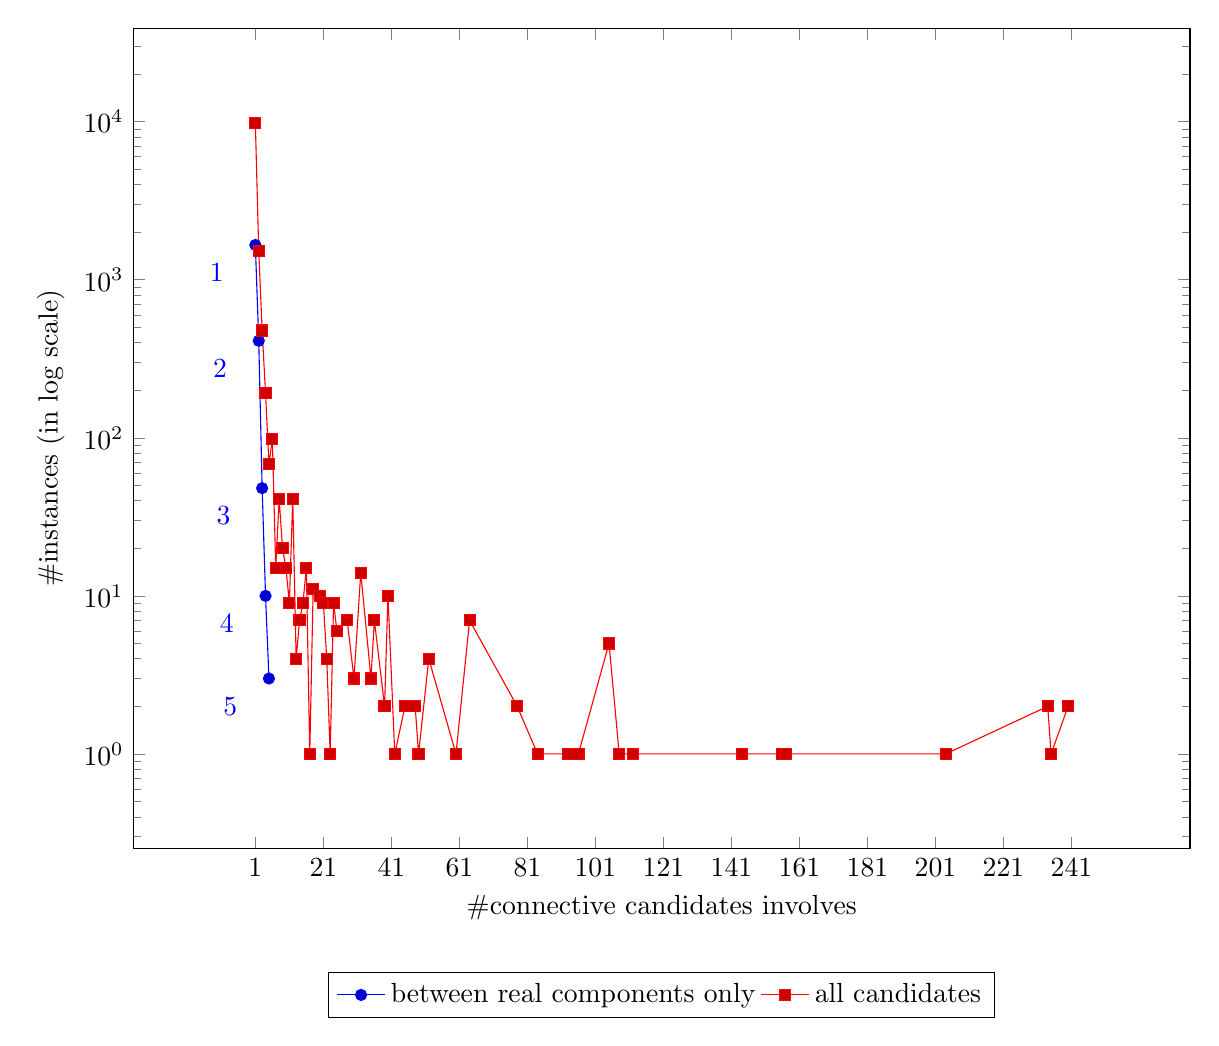
\begin{tikzpicture}
        \begin{axis}[
            width=15cm,
            height=12cm,
            enlargelimits=0.15,
            legend style={at={(0.5,-0.15)},
              anchor=north,legend columns=-1},
            xtick={1,21,...,245},
            xlabel={\#connective candidates involves},
            ylabel={\#instances (in log scale)},
            ymode=log,
            ]
        \addplot+[
                nodes near coords,
                every node near coord/.append style={xshift=-20, yshift=-10},
                nodes near coords align={horizontal},
                point meta=x,
                ] coordinates {
        (1,1659)
        (2,411)
        (3,48)
        (4,10)
        (5,3)
        };
        \addplot coordinates {
        (1,9827)
        (2,1525)
        (3,477)
        (4,191)
        (5,68)
        (6,98)
        (7,15)
        (8,41)
        (9,20)
        (10,15)
        (11,9)
        (12,41)
        (13,4)
        (14,7)
        (15,9)
        (16,15)
        (17,1)
        (18,11)
        (20,10)
        (21,9)
        (22,4)
        (23,1)
        (24,9)
        (25,6)
        (28,7)
        (30,3)
        (32,14)
        (35,3)
        (36,7)
        (39,2)
        (40,10)
        (42,1)
        (45,2)
        (48,2)
        (49,1)
        (52,4)
        (60,1)
        (64,7)
        (78,2)
        (84,1)
        (93,1)
        (96,1)
        (105,5)
        (108,1)
        (112,1)
        (144,1)
        (156,1)
        (157,1)
        (204,1)
        (234,2)
        (235,1)
        (240,2)
        };
        \legend{between real components only,all candidates}
        \end{axis}
    \end{tikzpicture}
\caption{\label{i:linking-ambig-chart} Number of connective candidates a component candidate involes. }
\end{figure}
